\chapter{CMS detector and LHC}
This thesis is done via analyzing the data collected by the Compact Muon Solenid (CMS) detector at the Large Hadron Collider (LHC). CMS is one of the two largest detectors built on the LHC. This chapter will briefly introduce the LHC and the CMS detector.

\section{Large Hadron Collider}
The LHC is the world's most powerful hadron collider and the largest experimental facility ever. It was built by the European Organization for Nuclear Research (CERN) between 1998 and 2008 in collaboration with over 10,000 scientists and engineers from over 100 countries, as well as hundreds of universities and laboratories. It lies in a tunnel 27 km in circumference, as deep as 175 m beneath the France$-$Switzerland border near Geneva. The designed maximum collison energy and highest luminosity of the LHC are 14 TeV and $\textup{10}^{-34} \textup{cm}^{-2}\textup{s}^{-1}$ respectively.\\
Other accelerators that had been originally built at CERN for previous experiments is working as an injection chain for the LHC now. The proton beam starts from LINAC, a small linear accelerator, where its energy firstly reaches 50 MeV. It then passes through a booster and goes to the PS, where it is accelerated up to 25 GeV. After that, it reaches 450 GeV in the SPS. The beam is finally injected in the LHC ring from the SPS, it is accelerated up to 4 TeV in 2012. In early 2015, the proton beam had been acceletated to 6.5 TeV, a value near its designed energy, before undergoing collision.\\
There are four collision points at the LHC, corresponding to four main experiments, CMS, ATLAS, LHCb and ALICE. The ALICE experiment is optimized to study heavy-ion (Pb-Pb nuclei) collisions and focusing on the physics of strongly interacting matter at extreme energy densities. LHCb is a specialized b-physics experiment, measuring the parameters of CP violation in the interactions of b-hadrons. Such studies can help to explain the matter-antimatter asymmetry of the universe. Last, CMS and ATLAS are two general purpose detectors. The aims of these two experiments are investigating a wide range of physics, including the search for the beyond standard model particles, extra dimensions, and dark matter.\\

\begin{figure}[hbtp]
  \begin{center}
    \includegraphics[width=0.9\textwidth]{figure/CH2/CERN_Overview.jpg}
  \end{center}
  \caption{\label{fig:LHC_overview}Overview of the LHC and relative location of the detectors.}
\end{figure}

\begin{figure}[hbtp]
  \begin{center}
    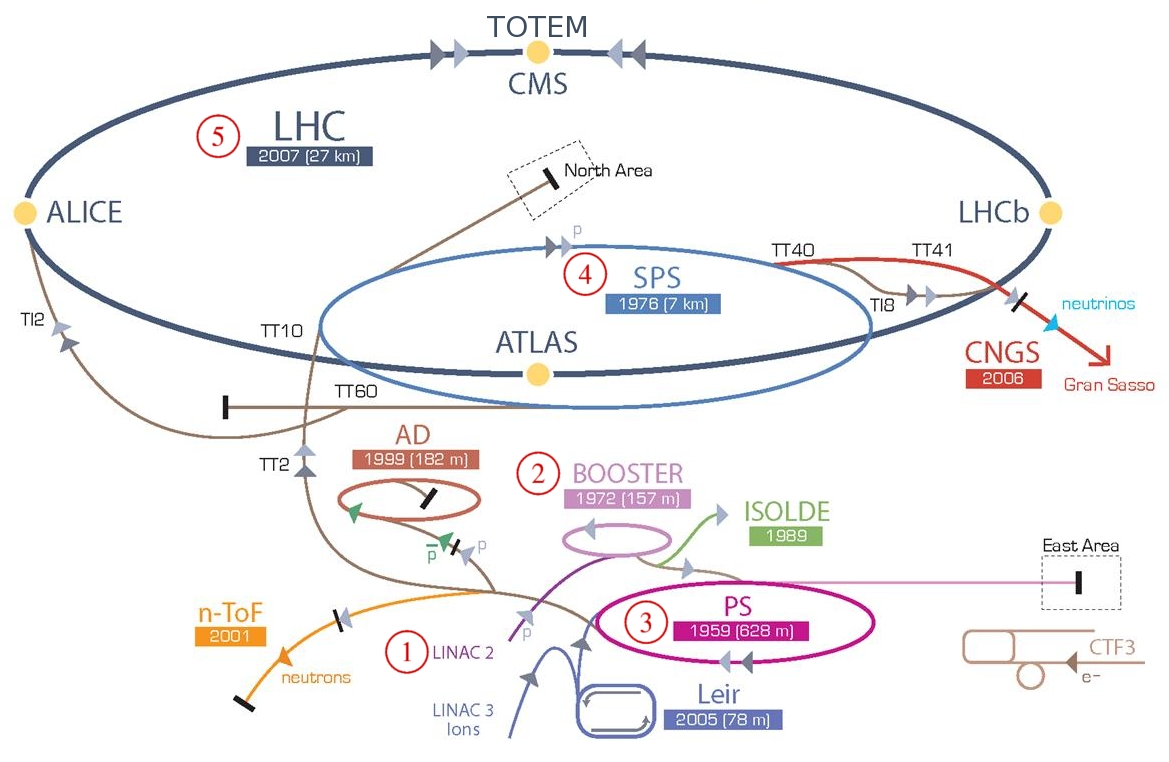
\includegraphics[width=0.9\textwidth]{figure/CH2/complex.png}
  \end{center}
  \caption{\label{fig:accelerator}CERN accelerator complex.}
\end{figure}

\section{Compact Muon Solenoid}
The Compact Muon Solenoid (CMS) detector is designed to cope very high rate of interactions expected to take place at the high LHC luminosity. It has the typical structure of detectors at hadron colliders: a central region ($barrel$) enclosed by two disks ($endcaps$). The structure of CMS can be seen in Fig.~(\ref{fig:CMS}).\\
\subsection*{Solenoid and Sub-detectors}
CMS features a powerful superconducting coil, generating a solenoidal magnetic field around 3.8 Tesla in a large volume, which hosts different sub-detctors. The magnetic field lines close through steel yoke in the outer region and the distinct sub-detectors are designed in order to obtain the highest possible resolution and the largest acceptance for every kind of particles.\\
The innermost layer is a silicon-based tracker. Surrounding it is a scintillating crystal electromagnetic calorimeter (ECAL), which is itself surrounded with a sampling calorimeter for hadrons (HCAL). The tracker and the calorimeters are compact enough to fit inside the CMS Solenoid. Outside the magnet are the large muon detectors separated by layers of the steel yoke.\\
\begin{figure}[hbtp]
  \begin{center}
    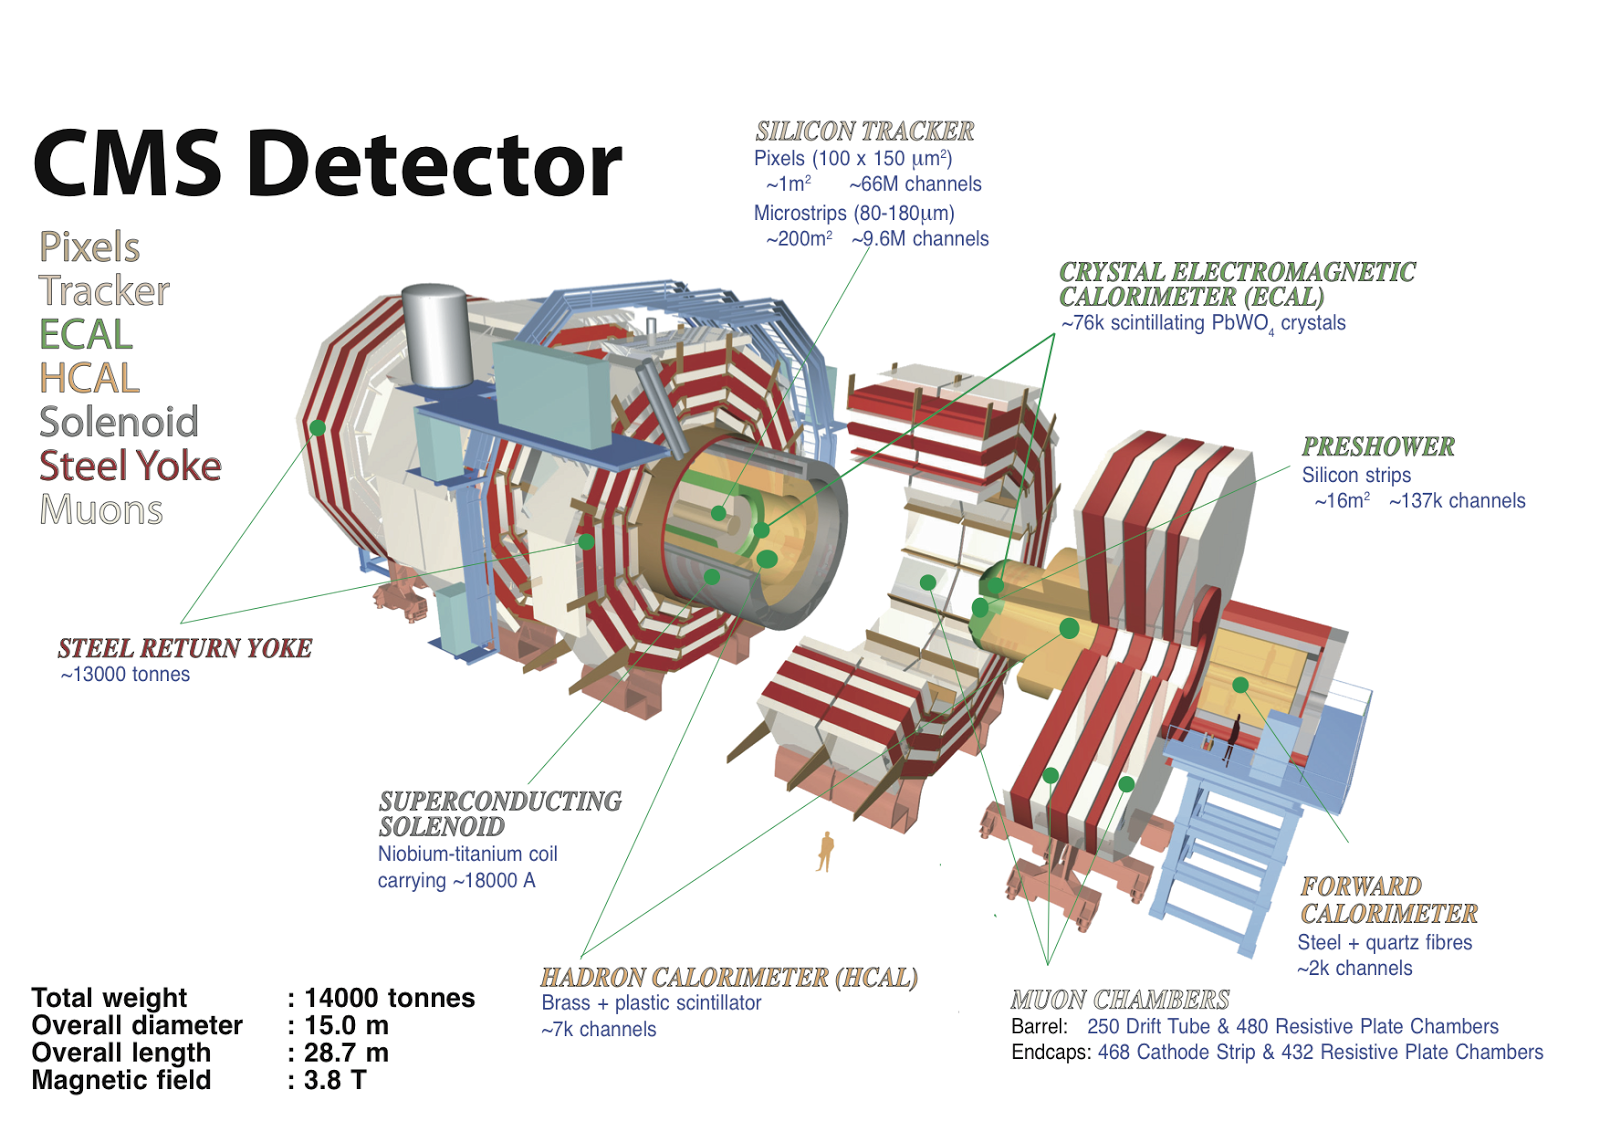
\includegraphics[width=0.9\textwidth]{figure/CH2/CMS.png}
  \end{center}
  \caption{\label{fig:CMS}Schematic layout of the CMS detector.}
\end{figure}
\subsection*{Coordinate System}
The CMS coordinate system is oriented such that the $x$-axis points to the center of the LHC ring, the $y$-axis points vertically upward and the $z$-axis is in the direction of the beam. The azimuthal angle $\phi$ is measured from the $x$-axis in the $xy$ plane and the radial coordinate in this plane is denoted by $r$. The polar angle $\theta$ is defined in the $rz$ plane, while the pseudo-rapidity $\eta=-ln\tan{(\theta/2)}$. The momentum component transverse to the beam direction, denoted by $p_{T}$, is computed from the $x$- and $y$-components, and the transverse energy is defined as $E_{T}=E\sin\theta$.

\subsection{Tracker}
\subsection{ECAL}
\subsection{HCAL}
\subsection{Muon Chamber}
\subsection{Trigger System}
